
%%%%%%%%%%%%%%%%%%%%%%%%%%%%%%%%%%%%%%%%%%%%

\section{Propriétés}

    \subsection{Mouvement rectiligne uniforme}

Lorsque nous sommes dans une automobile en mouvement rectiligne uniforme, nous ne ressentons pas le mouvement. Nous pouvons avoir l'impression que c'est le paysage qui est en mouvement.

 En revanche, lorsque l'automobile freine (mouvement non uniforme) ou prend un virage (mouvement non rectiligne), nous ressentons des {\it accélérations}.


\begin{center}
%%%%%%%%%%%%%%%%%%%%%%%%%%%%%%%%%%%%%%%%%%%%%%%%%%%%%%
%%%%%%%%%%%%%%%%%%%%%%%%%%%%%%%%%%%%%%%%%%%%%%%%%%%%%%%%%%%%%%%%%%%%
\def\scl{1}%scaling factor of the picture
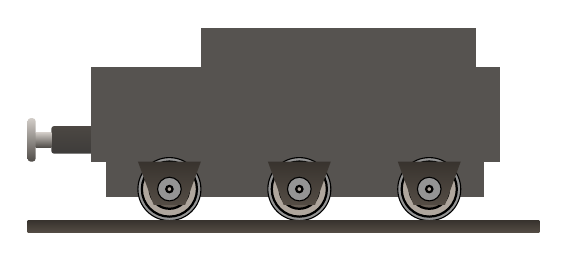
\begin{tikzpicture}[
  scale=\scl,
  tender/.style={gray!70!brown!20!black!75!},
  ]
%
%     TENDER
%
  \begin{scope}[xshift=0 cm,yshift=0 cm]

 % BUTOIR gauche
\def\hauteur{0.2}%
  \shade[bottom color=brown!10!gray!30!black!90!, top color=brown!20!gray!40!black!90!,rounded corners=1pt]
 (1.85, 0.9 + \hauteur) rectangle (0.3, 1.25 + \hauteur);
  \shade[bottom color=brown!10!gray!60!black, top color=brown!20!gray!40!]
 (0.3, 0.98 + \hauteur) rectangle (0.1, 1.17 + \hauteur);
  \shade[bottom color=brown!10!gray!60!black, top color=brown!20!gray!40!,rounded corners=1pt]
 (0, 0.8 + \hauteur) rectangle (0.1, 1.35 + \hauteur);

 % CORPS

    \fill[tender] (0.8, 1.0) rectangle (6.0, 2.2); % milieux

    \fill[tender] (2.2, 2.2) rectangle (5.7, 2.7); % haut

\def\hauteur{0.65} % hauteur des roues

    \fill[tender] (1.0,  \hauteur - 0.1) rectangle (5.8, 1.0); % bas

%  ROUES
  \foreach \x in {0, 1,..., 2}
 { \fill[black!20!gray!70!,draw=black,thin] (1.8 +\x * 1.65, \hauteur) circle (0.4 cm);
  \fill[brown!20!gray!70!,draw=black,thick] (1.8 +\x * 1.65, \hauteur) circle (0.35 cm);
  \fill[brown!20!black!70!,draw=black,thick] (1.8 +\x * 1.65, \hauteur) circle (0.25 cm); }

 % ESSIEUX
  \foreach \x in {0, 1,..., 2}
 { \shade[bottom color=brown!20!gray!60!black, top color=brown!20!gray!40!black]
 (1.6 +\x * 1.65, \hauteur -0.2) -- (2.0 +\x * 1.65, \hauteur -0.2) -- (2.2 +\x * 1.65, 1.0) -- (1.4 +\x * 1.65, 1.0) -- cycle;
  \fill[black!20!gray!70!,draw=black,thin] (1.8 +\x * 1.65, \hauteur) circle (0.15 cm);
  \fill[brown!20!gray!70!,draw=black,thick] (1.8 +\x * 1.65, \hauteur) circle (0.04 cm); }

  % RAIL
  \shade[bottom color=brown!20!gray!60!black, top color=brown!20!gray!40!black]
 (0, 0.25) rectangle (6.5, 0.1);

  \end{scope}
%
%
\end{tikzpicture}
%

\end{center}


  \subsection{Principe de relativité}

Énoncé par galilée au {\footnotesize XVII} $^\text{e}$ siècle, il exprime que les lois de la physique reste les mêmes dans  différents référentiels, en mouvement rectiligne uniforme les uns avec les autres.

    \subsubsection{Exemple}

On observe la chute d'une balle dans le champ de pesanteur. Elle est accélérée vers le bas et son mouvement est rectiligne. En reproduisant cette observation dans le train en mouvement rectiligne uniforme, le mouvement est identique.

  \subsection{Relativité des mouvements}

Le mouvements d'un objet dépend du référentiel dans lequel le mouvement est observé.

    \subsubsection{Additivité des vitesses}

Un train roule à la vitesse de 40 km/h. Un voyageur marche dans le couloir de ce train.
% à la vitesse de 5 km/h

\begin{center}
%%%%%%%%%%%%%%%%%%%%%%%%%%%%%%%%%%%%%%%%%%%%%%%%%%%%%%
%%%%%%%%%%%%%%%%%%%%%%%%%%%%%%%%%%%%%%%%%%%%%%%%%%%%%%%%%%%%%%%%%%%%
\def\scl{1}%scaling factor of the picture


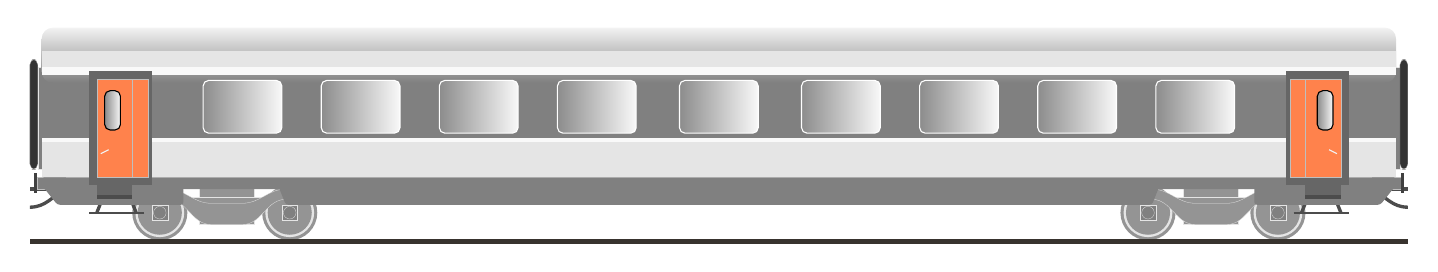
\begin{tikzpicture}[
  scale=\scl,
  %wagon/.style={yellow!30!brown!20!,rounded corners,draw=black,thick},
  wagon/.style={green!70!brown!20!black!75!,draw=black,thick},
 % toit/.style={black!70!brown!20!,draw=gray,thick},
  %roue/.style={brown!20!black!70!,draw=black,thick},
  fenetre/.style={white,rounded corners = 2pt,draw=black, thick},
  porte/.style={color=red!70!yellow!70!,draw=gray!50!, ultra thin}
  ]

  \begin{scope}[xshift=0 cm,yshift=0 cm]%, scale = 0.3
%
%         LIAISONS
% 
  \fill[color=gray,draw=gray!20!, ultra thin] % souflet gris
 (8.65, 0.9) rectangle (-8.65, 2.2);

 \draw[black!70!, very thick] 
    (8.3,0.65) to[out=330,in=180] (8.75,0.42);
 \draw[black!70!, very thick] 
    (-8.3,0.65) to[out=210,in=0] (-8.75,0.42);

  \foreach \t in {-1, 1}
  {
  \fill[color=black!80!,draw=gray!80!, ultra thin, rounded corners=2pt] % 
 (8.65 * \t, 0.9) rectangle (8.75 * \t, 2.3); % gris foncé, souflet

    \coordinate (A) at (8.3 * \t,0.65) ;
    \coordinate (B) at (8.75 * \t,0.65) ;
 \draw[black!70!, ultra thick] 
    (A) -- (B);

  }

 % BUTOIRS
  \foreach \t in {-1, 1}
  {
  \fill[color=gray,draw=gray!50!, ultra thin] % 
 (8.3 * \t, 0.65) rectangle (\t * 8.66, 0.8);
  \fill[color=gray!50!black] % 
 (\t * 8.66, 0.6) rectangle (\t * 8.7, 0.85);
  }
%
%     CORPS DU WAGON
%
  \shade[bottom color=gray, top color=gray!10!, rounded corners]  % toit
 (-8.6, 2) rectangle (8.6, 2.7);

  \fill[color=gray!20!] % gris clair
 (-8.6, 2.1) rectangle (8.6, 2.4);
  \fill[color=gray!20!] % gris clair
 (-8.6, 0.8) rectangle (8.6, 1.25);

  \fill[color=gray!5!] % blanc
 (-8.6, 2.1) rectangle (8.6, 2.2);
  \fill[color=gray!5!] % blanc
 (-8.6, 1.25) rectangle (8.6, 1.3);


% Arriere roues
  %\foreach \x in {6.25, -6.25} \fill[brown!40!black] (\x - 0.85, 0.8) rectangle (\x + 0.85, 0.45);

%  ROUES
\def\hauteur{0.35}% de l'axe des roues
\tikzset{
  roue/.pic={
    \fill[black!20!gray!70!] (0, \hauteur) circle (0.35 cm);
    \fill[gray!20!] (0, \hauteur) circle (0.31 cm);
    \fill[black!20!gray!70!] (0, \hauteur) circle (0.28 cm);

  \fill[color=gray,draw=gray!20!, ultra thin] %,rotate=45
 (0.1, \hauteur + -0.1) rectangle (-0.1, \hauteur + 0.1);

  \fill[color=gray,draw=gray!20!, ultra thin] (0, \hauteur) circle (0.08 cm);

  }
}

  \pic at (5.45,0)    {roue};
  \pic at (7.1,0)    {roue};
  \pic at (-5.45,0)    {roue};
  \pic at (-7.1,0)    {roue};
 % ESSIEUX
\def\y{0.2}
  \foreach \x in {6.25, -6.25}
   {
 \fill[black!20!gray!70!,draw=gray!20!, ultra thin] 
  (\x - 0.35, 0.2) rectangle (\x + 0.35, 0.45);

 \fill[black!20!gray!70!,draw=gray!20!, ultra thin] 
  (\x - 0.45, 0.45) rectangle (\x + 0.45, 0.55);

 \fill[black!20!gray!70!,draw=gray!20!, ultra thin] 
  (\x - 0.35, 0.55) rectangle (\x + 0.35, 0.7);

    \coordinate (A) at (\x + -0.75,\y + 0.45) ;
      \coordinate (B) at (\x - 0.2,\y + 0.27) ;
      \coordinate (C) at (\x + 0.2,\y + 0.27) ;
    \coordinate (D) at (\x + 0.75,\y + 0.45) ;
    \coordinate (E) at (\x + 0.75,\y + 0.32) ;
      \coordinate (F) at (\x + 0.2,\y + 0) ;
      \coordinate (G) at (\x - 0.2,\y + 0) ;
    \coordinate (H) at (\x - 0.75,\y + 0.32) ;
 \fill[black!20!gray!70!,draw=gray!20!, ultra thin] 
    (A) to[out=0,in=180] (B) to[out=0,in=180] (C) to[out=0,in=180]
    (D) to[out=-90,in=90] (E) to[out=180,in=0] (F) to[out=180,in=0]
    (G) to[out=180,in=0] (H) -- cycle;
  }

% MARCHE
  \foreach \t in {-1, 1}
  {
    \draw[draw=black!70!,very thick] % montant
 (\t * 7.9, 0.35) -- (\t * 7.8, 0.6);
    \draw[draw=black!70!,very thick] % montant
 (\t * 7.4, 0.35) -- (\t * 7.5, 0.6);
    \draw[draw=black!70!,thick] % marche
 (\t * 7.3, 0.35) -- (\t * 8, 0.35);
  }

% BAS DE CAISSE

  \fill[color=gray, rounded corners=1pt] % gris Foncé
    (-8.6, .8) rectangle (8.6, .65);


  \foreach \t in {-1, 1}
  \fill[color=gray, rounded corners=1pt] % gris Foncé
    (\t * 8.6, .7) -- (\t * 8.4, .45) -- (\t * 6.8, .45) -- (\t * 6.8, .7) -- cycle;
  \fill[color=gray, rounded corners=1pt] % gris Foncé
    (5.6, .7) -- (5.5, .45) -- (-5.5, .45) -- (-5.6, .7) -- cycle;

      % FENÊTRES
  \foreach \t in {1.05, 2.55, 4.05, 5.55}
  {
  \shade[bottom color=gray!5!, top color=gray!90!, shading angle={90},rounded corners=2pt, draw=white]
   (\t, 1.36) rectangle (\t + 1, 2.03);
  \shade[bottom color=gray!5!, top color=gray!90!, shading angle={90},rounded corners=2pt, draw=white]
   (-\t, 1.36) rectangle (-\t - 1, 2.03);
  }
  \shade[bottom color=gray!5!, top color=gray!90!, shading angle={90},rounded corners=2pt, draw=white]
   (-0.5, 1.36) rectangle (0.5, 2.03);

      % PORTES
  \foreach \t in {-1, 1}
  {

    \fill[gray!80!black] % marche
 (\t * 7.45, 0.53) rectangle (\t * 7.9, 0.7);
    \fill[gray!60!black] % marche
 (\t * 7.45, 0.53) rectangle (\t * 7.9, 0.57);

  \fill[gray!80!black]
 (\t * 7.2, 0.7) rectangle (\t * 8, 2.15);
  \fill[porte]
 (\t * 7.25, 0.8) rectangle (\t * 7.6, 2.05);
  \fill[porte]
 (\t * 7.45, 0.8) rectangle (\t * 7.9, 2.05);

  \shade[bottom color=gray!5!, top color=gray!90!, shading angle={90},rounded corners=2pt, draw=black] % fenêtre
   (\t * 7.6, 1.4) rectangle (\t * 7.8, 1.9);

    \draw[gray!10!]
 (\t * 7.75, 1.15) -- (\t * 7.85, 1.1); % poignée
  }

  % RAIL
  \fill[color=brown!20!gray!40!black]
 (-8.75, 0.02) rectangle (8.75, -0.05);

  \end{scope}
%
%
\end{tikzpicture}
%

\end{center}
%Un voyageur marche dans le couloir d'un train à la vitesse de 5 km/h. Le train roulant à la vitesse de 100 km/h. 

Pour un observateur dans le référentiel terrestre, le train a une vitesse de 40 km/h et le voyageur a une vitesse de 45 km/h. 

Le voyageur a une vitesse de 5 km/h dans le référentiel du train.

    \subsubsection{Relativité des trajectoires}

Dans le référentiel du train, la chute d'une balle lachée par un voyageur est rectiligne.

Dans le référentiel terrestre, la trajectoire de la balle est une courbe.

%%  \subsection{}

%%%%%%%%%%%%%%%%%%%%%%%%%%%%%%%%%%%%%%%%%%%{\it }



